% =====================================================================
%  Informe de entregables de Sebastián — Efecto Mpemba cuántico
%  Documento maestro que ENSAMBLA los fragmentos \input-ables de cada
%  entregable (items 3, 4, 5 y 8). Las rutas de figura de los fragmentos
%  son relativas a este directorio (context/doc/), por lo que ESTE .tex
%  debe compilarse DESDE context/doc/:
%
%    cd context/doc
%    pdflatex informe_sebastian_entregables
%    pdflatex informe_sebastian_entregables      % (2x para el índice)
%
%  El PDF final se publica en mpemba-cuantico/informe_sebastian_entregables.pdf
% =====================================================================
\documentclass[11pt,a4paper]{article}

\usepackage[utf8]{inputenc}
\usepackage[T1]{fontenc}
\usepackage{babel}
\babelprovide[import,main]{spanish}
\usepackage{amsmath,amssymb,amsthm}
\usepackage{physics}
\usepackage{bm}
\usepackage{geometry}
\geometry{margin=2.4cm}
\usepackage{graphicx}
\usepackage{booktabs}
\usepackage{algorithm}
\usepackage{algpseudocode}
\usepackage{xcolor}
\usepackage{mdframed}
\usepackage{enumitem}
\usepackage{listings}
\usepackage[hidelinks,colorlinks=true,linkcolor=blue!55!black,citecolor=teal!60!black,urlcolor=blue!55!black]{hyperref}

% --- Estilo para listados de codigo (Python / C++) ---
\definecolor{codegray}{rgb}{0.5,0.5,0.5}
\definecolor{codegreen}{rgb}{0.0,0.45,0.18}
\definecolor{codeblue}{rgb}{0.10,0.20,0.6}
\definecolor{codered}{rgb}{0.65,0.12,0.12}
\definecolor{codebg}{rgb}{0.975,0.975,0.975}
\lstdefinestyle{qmpe}{
  backgroundcolor=\color{codebg},
  basicstyle=\ttfamily\scriptsize,
  commentstyle=\color{codegreen}\itshape,
  keywordstyle=\color{codeblue}\bfseries,
  stringstyle=\color{codered},
  numberstyle=\tiny\color{codegray},
  numbers=left, numbersep=5pt,
  breaklines=true, breakatwhitespace=false,
  showstringspaces=false, tabsize=2, captionpos=b,
  frame=single, rulecolor=\color{codegray!40},
}
\lstset{style=qmpe}

\theoremstyle{definition}
\newtheorem{definicion}{Definición}[section]
\theoremstyle{plain}
\newtheorem{teorema}{Teorema}[section]
\newtheorem{proposicion}{Proposición}[section]
\newtheorem{observacion}{Observación}[section]

\newcommand{\Lop}{\mathcal{L}}
\newcommand{\Ldual}{\mathcal{L}^{\dagger}}
\newcommand{\Dop}{\mathcal{D}}
\newcommand{\Hs}{\mathcal{H}}
\newcommand{\rss}{\rho_{\mathrm{ss}}}
\renewcommand{\Tr}{\operatorname{Tr}}
\newcommand{\vecop}[1]{\operatorname{vec}\!\left(#1\right)}

\newmdenv[linecolor=teal!55!black,linewidth=0.8pt,backgroundcolor=teal!4,
  roundcorner=4pt,skipabove=8pt,skipbelow=8pt,innertopmargin=6pt,innerbottommargin=6pt]{cajaclave}

\title{\textbf{Entregables de Sebastián --- Efecto Mpemba cuántico}\\
\large items 3, 4, 5 y 8: evolución temporal (a/b), trayectorias y relevancia macro}
\author{Sebastián}
\date{\today}

\begin{document}
\maketitle
\begin{center}\itshape\small
Documento de revisión. Cada sección se \texttt{\textbackslash input} en el maestro
\texttt{mpemba\_cuantico.tex}.
\end{center}
\tableofcontents
\bigskip

% =====================================================================
%  Entregable T2(a): Evolucion temporal por integracion directa (RK4)
%  Fragmento \input-able en el documento maestro (context/doc/mpemba_cuantico.tex).
%  Las figuras se referencian relativas a context/doc/.
% =====================================================================
\section{Evolución temporal (a): integración directa con RK4}
\label{sec:t2a}

\subsection{Explicación del framework}
La tarea de \emph{evolución temporal} consiste en obtener la trayectoria del
operador densidad $\rho(t)$ que resuelve la ecuación maestra de Lindblad
$\dot\rho=\mathcal{L}[\rho]$ (ec.~\eqref{eq:gksl}) a partir de una preparación
$\rho_0$, para trazar las curvas de distancia al equilibrio
$\Dop(\rho_t\|\rss)$ que revelan (o descartan) el efecto Mpemba. El método~(a)
es la vía \textbf{directa}: integrar la ecuación diferencial paso a paso, sin
construir el superoperador $\mathbb{L}$ de dimensión $d^2\times d^2$, aplicando
en su lugar la acción \emph{matrix-free}
$\mathcal{L}[\rho]=-i[H,\rho]+\sum_\mu(L_\mu\rho L_\mu^\dagger-\tfrac12\{L_\mu^\dagger L_\mu,\rho\})$.

\subsection{Discretización y método numérico}
Se emplea el método de \textbf{Runge--Kutta clásico de 4.º orden} (RK4), un
integrador explícito de un paso. Para $\dot\rho=\mathcal{L}[\rho]$ y paso
$\Delta t$:
\begin{align*}
k_1&=\mathcal{L}[\rho_n], &
k_2&=\mathcal{L}[\rho_n+\tfrac{\Delta t}{2}k_1], &
k_3&=\mathcal{L}[\rho_n+\tfrac{\Delta t}{2}k_2], \\
k_4&=\mathcal{L}[\rho_n+\Delta t\,k_3], &
\rho_{n+1}&=\rho_n+\tfrac{\Delta t}{6}(k_1+2k_2+2k_3+k_4). &&
\end{align*}
El error local es $\mathcal{O}(\Delta t^5)$ y el global $\mathcal{O}(\Delta t^4)$.
Cada paso requiere \emph{cuatro} evaluaciones del Liouvilliano; cada evaluación,
para la cadena de Ising disipativa, son $2+3N_J$ productos de matrices densas
$d\times d$ (con $N_J=2N$ operadores de salto), de coste $\mathcal{O}(d^3)$ cada
uno. El coste por paso es por tanto $\mathcal{O}(N\,d^3)$.

\subsection{Implementación serial}
El núcleo está en \texttt{common/lindblad.hpp} (acción \texttt{apply\_lindblad},
modelo \texttt{build\_ising}, estado de Gibbs por tiempo imaginario) y el
integrador en \texttt{a\_integracion\_directa/src/rk4\_evolution.cpp}. La
preparación inicial es un estado de Gibbs a $T_0=5$ y la referencia de relajación
el estado de Gibbs del baño a $T=0{,}8$. El \emph{hotspot} absoluto es el
producto de matrices densas \texttt{matmul}.

\subsection{Justificación de la paralelización: OpenMP}
El patrón de cómputo de la integración directa es: \emph{miles de pasos
secuenciales} (dependencia temporal estricta: $\rho_{n+1}$ necesita $\rho_n$),
cada uno dominado por productos de matrices densas que reutilizan los mismos
datos. La dependencia temporal \textbf{impide} paralelizar entre pasos; el
paralelismo disponible está \emph{dentro} de cada paso, en el \texttt{matmul}.
Ese es un patrón de \textbf{memoria compartida} con datos regulares y de tamaño
moderado ($d\times d$ cabe en caché/RAM de un nodo): el paradigma natural es
\textbf{OpenMP}, paralelizando el bucle de filas del \texttt{matmul}
(\texttt{\#pragma omp parallel for}). MPI sería contraproducente aquí
(distribuir matrices pequeñas introduce comunicación de halo en cada uno de los
miles de pasos); CUDA daría más ancho de banda pero no hay GPU disponible en la
máquina de prueba (se discute como trabajo futuro en \S\ref{sec:t2b} y en la
tabla~\ref{tab:paradigma}). La corrección de la versión paralela se verifica de
forma exacta: serial y multinúcleo producen el \emph{mismo} estado final
(coincidencia a precisión de máquina del observable $D_{HS}$ final).

\subsection{Comparación serial vs paralelo}
\begin{figure}[h]
\centering
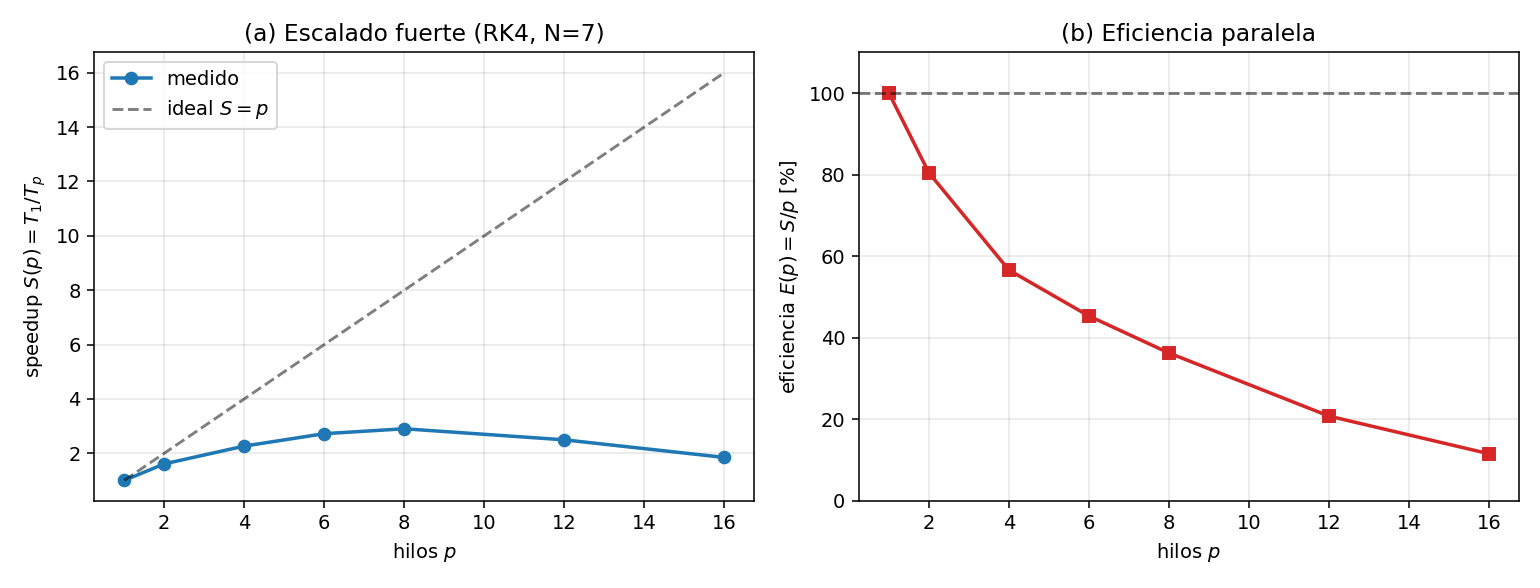
\includegraphics[width=0.92\textwidth]{../../T2/a_integracion_directa/results/fig_t2a_speedup.png}
\caption{Escalado fuerte del integrador RK4 (cadena de Ising disipativa $N=7$,
$d=128$) en un AMD Ryzen 7 7730U (8 núcleos físicos / 16 hilos). (a) speedup
$S(p)=T_1/T_p$ frente al ideal $S=p$; (b) eficiencia paralela $E(p)=S/p$.}
\label{fig:t2a_speedup}
\end{figure}

El speedup es \textbf{sublineal} y satura cerca del número de núcleos físicos: se
alcanza $S_{\max}\approx2{,}9$ con $8$ hilos, con eficiencia del
$36\,\%$ a 8 hilos. El ajuste a la \textbf{ley de Amdahl}
$S(p)=1/[f+(1-f)/p]$ da una fracción serie efectiva $f\approx0{,}25$. Las
causas de la sublinealidad son típicas de este patrón: (i)~el integrador hace
\emph{fork/join} de OpenMP en cada uno de los muchos \texttt{matmul} pequeños,
con sobrecoste acumulado; (ii)~el problema es \emph{memory-bandwidth bound}
(las matrices se releen de memoria), de modo que los hilos compiten por el
ancho de banda compartido; (iii)~las asignaciones de memoria temporales y las
operaciones vectoriales fuera del \texttt{matmul} son seriales. El salto de 8 a
16 hilos aporta poco porque los 16 hilos son \emph{hyperthreads} sobre 8 núcleos
físicos, sin ancho de banda adicional.

Para ver \emph{directamente} la mejora —y no solo el speedup adimensional— la
Figura~\ref{fig:t2a_serial_parallel} enfrenta el \textbf{tiempo de cómputo en
serie (1~hilo) y en paralelo (8~hilos)} en función del tamaño del sistema~$N$
(la malla del operador, $d=2^N$), a igual número de pasos. Ambas curvas crecen
como $\sim d^3$, pero la paralela queda sistemáticamente por debajo: la
\emph{separación} entre las dos es la ganancia, y crece con la malla porque a
mayor $d$ el \texttt{matmul} domina y amortiza mejor el coste de \emph{fork/join}.

\begin{figure}[h]
\centering
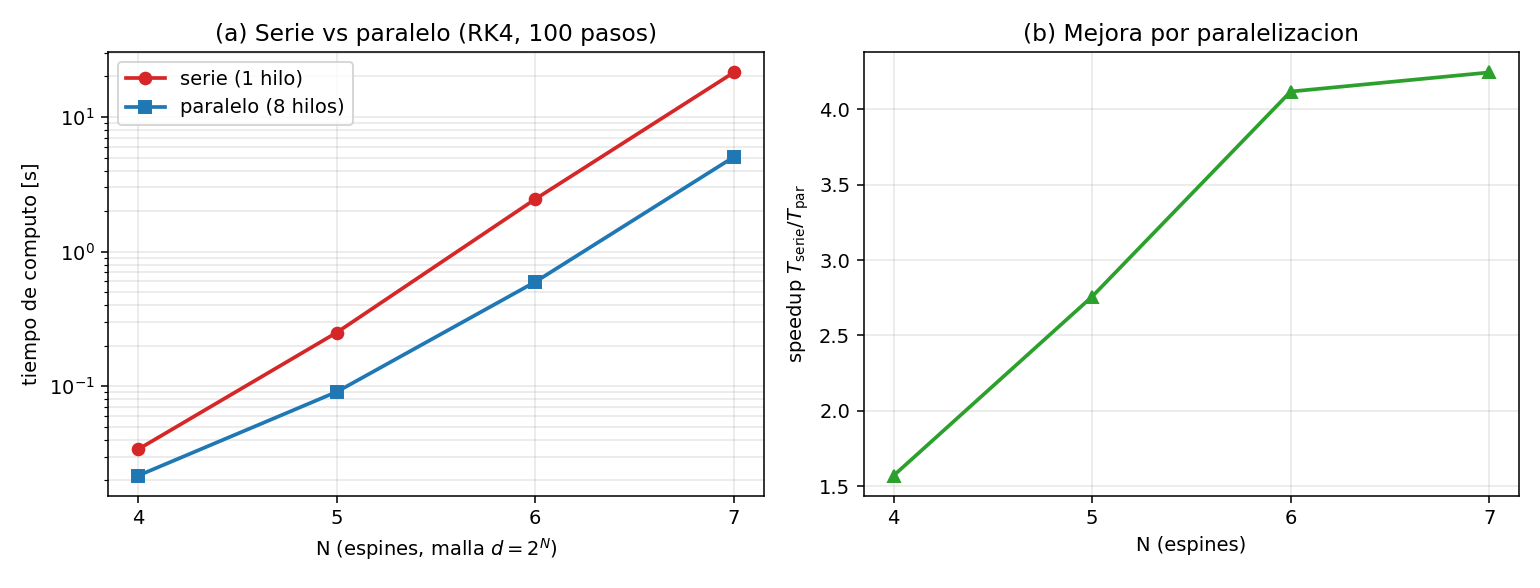
\includegraphics[width=0.92\textwidth]{../../T2/a_integracion_directa/results/fig_t2a_serial_parallel.png}
\caption{Tiempo de cómputo \textbf{serie vs paralelo} del RK4 frente al tamaño
del sistema $N$ (malla $d=2^N$), a $100$ pasos fijos. (a)~las dos curvas
($1$~hilo en rojo, $8$~hilos en azul, escala log) muestran el mismo coste
$\sim d^3$ desplazado: el hueco entre ellas es la mejora. (b)~el speedup
$T_{\mathrm{serie}}/T_{\mathrm{par}}$ resultante crece con la malla (de
$\sim\!1{,}6$ en $N=4$ a $\sim\!4$ en $N=7$): cuanto mayor es $d$, más domina el
\texttt{matmul} y mejor se amortiza el \emph{fork/join}, aunque siempre sublineal
frente al ideal de $8$.}
\label{fig:t2a_serial_parallel}
\end{figure}

\subsection{Resultados y validación}
\paragraph{Correctitud y orden del método.}
La figura~\ref{fig:t2a_convergence} valida el integrador frente a la evolución
espectral \emph{exacta} $e^{t\mathcal{L}}\rho_0$ (suma de modos): el error a
tiempo fijo decae como $\Delta t^4$, confirmando el \textbf{orden 4} del RK4
(pendiente medida $\approx4{,}04$).

\begin{figure}[h]
\centering
\begin{minipage}{0.49\textwidth}\centering
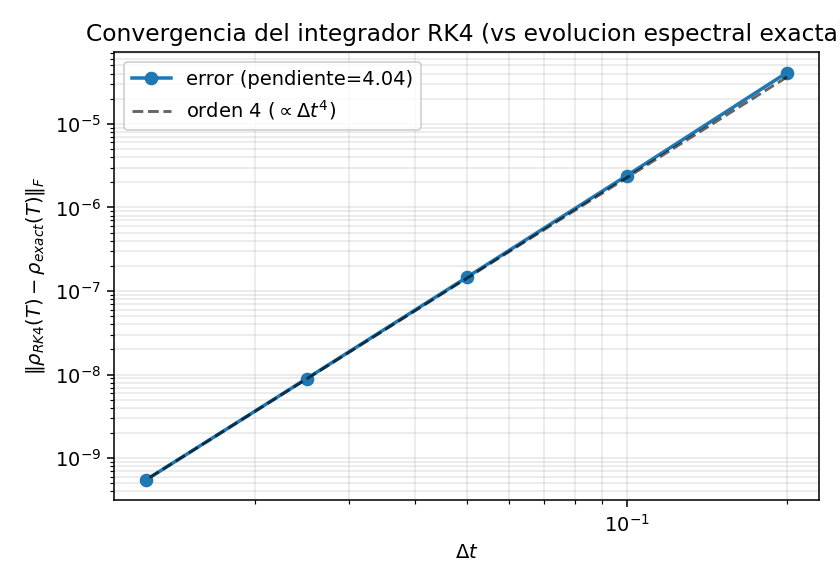
\includegraphics[width=\textwidth]{../../T2/a_integracion_directa/results/fig_t2a_convergence.png}
\end{minipage}\hfill
\begin{minipage}{0.49\textwidth}\centering
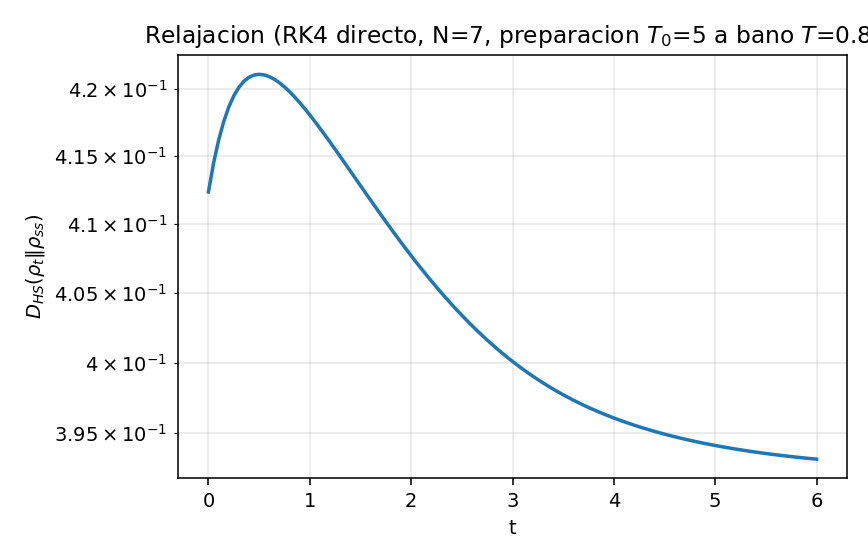
\includegraphics[width=\textwidth]{../../T2/a_integracion_directa/results/fig_t2a_relax.png}
\end{minipage}
\caption{Izquierda: convergencia de orden 4 del RK4 frente a la solución exacta.
Derecha: curva de relajación $D_{HS}(t)$ producida por el método (preparación
caliente $T_0=5$ relajando al baño $T=0{,}8$).}
\label{fig:t2a_convergence}
\end{figure}

\paragraph{Coste con el tamaño.}
La figura~\ref{fig:t2a_size} confirma el escalado $\mathcal{O}(d^3)$ por paso esperado
del producto de matrices densas: al pasar de $N$ a $N+1$ ($d\to2d$) el coste por
paso se multiplica por $\sim 8$. Es justamente este crecimiento el que vuelve
inviable la representación densa de $\rho$ para $N$ grande y motiva las
trayectorias (\S\ref{sec:t3}) en el régimen de muchos cuerpos.

\begin{figure}[h]
\centering
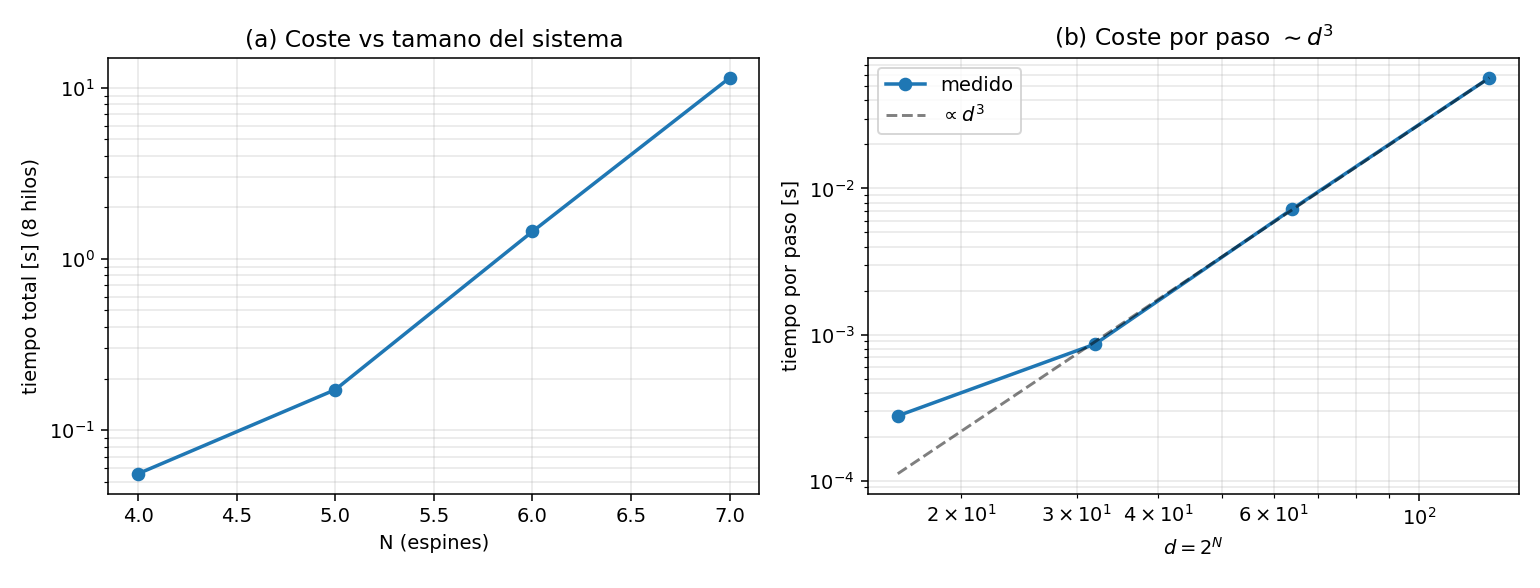
\includegraphics[width=0.92\textwidth]{../../T2/a_integracion_directa/results/fig_t2a_size.png}
\caption{Coste del método con el tamaño del sistema (8 hilos). (a) tiempo total;
(b) tiempo por paso frente a la referencia $\propto d^3$.}
\label{fig:t2a_size}
\end{figure}

\paragraph{Conclusión del método (a).}
La integración directa por RK4 es \emph{simple, exacta a orden 4 y robusta}, y se
paraleliza de forma natural con OpenMP a nivel del producto de matrices. Su
limitación es doble: el coste $\mathcal{O}(d^3)$ por paso y la necesidad de pasos
pequeños por estabilidad/precisión, que obligan a muchas evaluaciones del
Liouvilliano. El método~(b) (acción del exponencial, \S\ref{sec:t2b}) ataca
precisamente este segundo punto.

% =====================================================================
%  Entregable T2(b): Evolucion temporal por accion del exponencial (Krylov)
%  Fragmento \input-able en context/doc/mpemba_cuantico.tex
% =====================================================================
\section{Evolución temporal (b): acción del exponencial por Krylov}
\label{sec:t2b}

\subsection{Explicación del framework}
El método~(b) resuelve la misma evolución $\dot\rho=\mathcal{L}[\rho]$ pero por una
vía distinta: en lugar de integrar paso a paso, aproxima directamente la
\textbf{acción del exponencial del Liouvilliano},
\[
\rho(t+\tau)=e^{\tau\mathcal{L}}[\rho(t)],
\]
que es la solución \emph{exacta} en un paso de tamaño $\tau$. La dificultad es que
$e^{\tau\mathcal{L}}$ es un objeto de dimensión $d^2\times d^2$ imposible de
formar. La idea de Krylov es proyectar la acción sobre el subespacio
$\mathcal{K}_m=\text{span}\{\rho,\mathcal{L}\rho,\dots,\mathcal{L}^{m-1}\rho\}$,
de dimensión $m\ll d^2$, donde el exponencial es trivial de calcular.

\subsection{Del modelo teórico a la discretización (paso a paso)}
\label{ssec:t2b_discr}

\paragraph{Paso 0 — Modelo teórico.} El mismo de~(a): la ecuación maestra GKSL
$\dot\rho=\Lop[\rho]$ para la cadena de Ising disipativa (Hamiltoniano $H$ y
canales $L_\mu$ idénticos, \S\ref{ssec:t2a_discr}).

\paragraph{Paso 1 — Solución formal exacta.} En lugar de integrar la EDO, se usa
que la solución del PVI es \emph{exacta} en un paso de tamaño $\tau$ mediante el
exponencial del generador:
\[
\rho(t+\tau)=e^{\tau\Lop}[\rho(t)].
\]
El obstáculo: $e^{\tau\Lop}$ vive en el superoperador de dimensión
$d^2\times d^2$, imposible de formar y exponenciar para $N$ grande.

\paragraph{Paso 2 — Discretización por proyección de Krylov (Arnoldi).} Se proyecta
la acción del exponencial sobre el subespacio de Krylov
$\mathcal{K}_m=\text{span}\{\rho,\Lop\rho,\dots,\Lop^{m-1}\rho\}$ ($m\ll d^2$). Con
\textbf{Arnoldi} se construye una base ortonormal $\{Q_0,\dots,Q_{m-1}\}$ (cada
$Q_i$ es un operador $d\times d$; producto interno de Frobenius
$\langle A,B\rangle=\Tr(A^\dagger B)$) y la matriz de Hessenberg
$H_m\in\mathbb{C}^{m\times m}$ que representa $\Lop$ en esa base. El \emph{único}
ingrediente que toca el sistema grande es la acción $w=\Lop[Q_j]$ en cada
iteración de Arnoldi.

\paragraph{Paso 3 — Exponencial pequeño y reconstrucción.} La acción discretizada es
\[
e^{\tau\Lop}[\rho]\;\approx\;\|\rho\|_F\;\sum_{i=0}^{m-1}\big[e^{\tau H_m}\big]_{i,0}\,Q_i,
\]
con $e^{\tau H_m}$ calculado sobre la matriz \emph{pequeña} $m\times m$ por
\emph{scaling-and-squaring} con serie de Taylor (\texttt{small\_expm}). Coste por
bloque: $m$ aplicaciones de $\Lop$ (Arnoldi) $+\,\mathcal{O}(m\,d^2)$ y un
$e^{\tau H_m}$ de coste $\mathcal{O}(m^3)$ despreciable. La ventaja decisiva: para
$\tau$ dentro del radio de convergencia, $m\sim20$--$30$ basta para precisión de
máquina y \emph{un solo bloque avanza un paso de tiempo grande}.

\subsection{Implementación serial y líneas de código}
En \texttt{b\_accion\_exponencial/src/krylov\_evolution.cpp}. El bucle de Arnoldi
(Paso~2) es el corazón del método; nótese que cada iteración llama a la misma
acción \texttt{apply\_lindblad} de~(a) —es decir, \emph{comparte el hotspot
paralelizable}—:

\begin{lstlisting}[language=C++,caption={Bucle de Arnoldi de \texttt{krylov\_step} (\texttt{krylov\_evolution.cpp}): la línea \texttt{apply\_lindblad(...)} es la acción matrix-free de $\mathcal L$, donde se cuenta el trabajo (\texttt{L\_applies}) y donde reside la paralelización OpenMP (vía \texttt{matmul}, Listado~\ref{lst:t2b_omp}).},label={lst:t2b_arnoldi}]
for (int j = 0; j < m; ++j) {
    Mat w = apply_lindblad(H, Ls, Lds, LdL, Q[j], d); ++L_applies;   // <-- hotspot (OpenMP)
    for (int i = 0; i <= j; ++i) {                       // ortogonalizacion de Gram-Schmidt
        cd hij = fro_dot(Q[i], w); Hess[i*m+j] = hij; axpy(w, Q[i], -hij);
    }
    double hj = fro_norm(w);
    Hess[(j+1)*m+j] = hj;
    if (hj < 1e-12) { mm = j + 1; break; }               // convergencia anticipada
    Q.push_back(scaled(w, 1.0 / hj));
}
\end{lstlisting}

\subsection{La directiva de paralelización (OpenMP)}
El \emph{hotspot} es el mismo que en~(a): el producto de matrices densas, llamado
$m$ veces por bloque dentro de \texttt{apply\_lindblad}. La directiva es por tanto
idéntica —una sola \texttt{\#pragma omp parallel for} en \texttt{matmul}
(\texttt{common/lindblad.hpp})—, lo que explica que el escalado paralelo de~(b)
sea equivalente al de~(a):

\begin{lstlisting}[language=C++,caption={La misma directiva OpenMP que en T2(a): el bucle de filas de \texttt{matmul} es el único punto paralelizado (compartido por RK4 y Krylov).},label={lst:t2b_omp}]
    #pragma omp parallel for schedule(static)   // <-- DIRECTIVA: filas i repartidas entre hilos
    for (int i = 0; i < d; ++i)
        for (int k = 0; k < d; ++k) { /* C[i,:] += A[i,k] * B[k,:] */ }
\end{lstlisting}

\subsection{Justificación de la paralelización: OpenMP}
Como en el método~(a), el \emph{hotspot} es la acción $\mathcal{L}[\cdot]$ (el
producto de matrices densas), llamada $m$ veces por bloque. La ortogonalización
de Arnoldi añade productos internos de Frobenius de coste $\mathcal{O}(d^2)$,
mucho menores que el $\mathcal{O}(d^3)$ del \texttt{matmul}. Por tanto el patrón
sigue siendo de \textbf{memoria compartida} dominado por \texttt{matmul}, y el
paradigma natural vuelve a ser \textbf{OpenMP} sobre el mismo bucle. (En el
régimen de muchos cuerpos, donde $d^2$ no cabe en memoria, la acción de Krylov se
paraleliza con MPI distribuyendo el vector $\ket{\rho}\rangle$; aquí, con $\rho$
denso en un nodo, OpenMP es lo adecuado.) La corrección se verifica de dos formas:
serial y paralelo dan el mismo resultado, y el resultado coincide con el del
método~(a) (RK4) a todas las cifras: $D_{HS}^{\text{final}}=0{,}4241128226$ para
$N=6$, idéntico por ambos métodos (referencia exacta por evolución espectral:
$D_{HS}^{\text{exacto}}=0{,}42411283$).

\subsection{Comparación serial vs paralelo}
\begin{figure}[h]
\centering
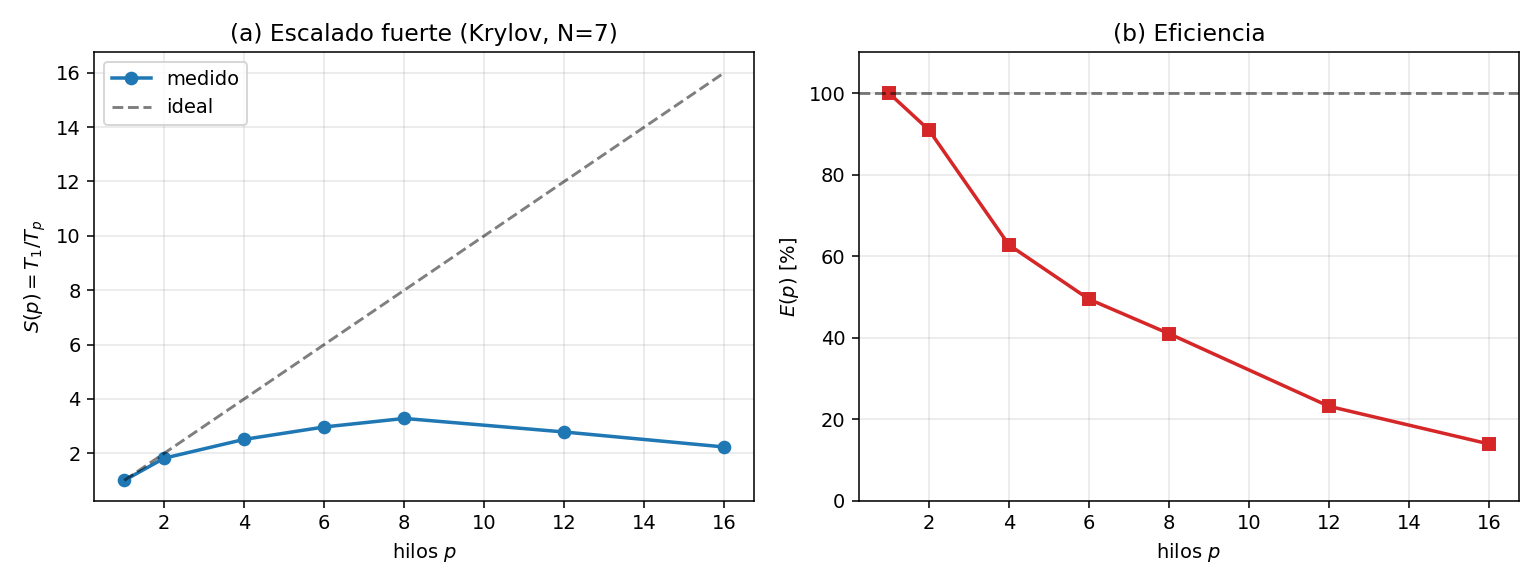
\includegraphics[width=0.92\textwidth]{../../T2/b_accion_exponencial/results/fig_t2b_speedup.png}
\caption{Escalado fuerte del método de Krylov (Ising disipativo $N=7$, $d=128$).
El comportamiento es análogo al del método~(a): speedup sublineal que satura en
los núcleos físicos, por las mismas causas (fork/join del \texttt{matmul},
\emph{memory-bandwidth bound}, hyperthreading sin ancho de banda extra). Pico
$S_{\max}\approx3{,}3$, eficiencia $41\,\%$ a 8 hilos (ligeramente mejor que
RK4: hay menos llamadas a \texttt{matmul} por unidad de trabajo).}
\label{fig:t2b_speedup}
\end{figure}

La Figura~\ref{fig:t2b_serial_parallel} muestra la mejora de forma directa: el
\textbf{tiempo de cómputo en serie (1~hilo) frente al paralelo (8~hilos)} en
función del tamaño del sistema~$N$ (malla $d=2^N$), a igual paso $\tau$ y misma
dimensión de Krylov $m$. Igual que en~(a), las dos curvas crecen como $\sim d^3$
y el hueco entre ellas —la ganancia— se ensancha con la malla.

\begin{figure}[h]
\centering
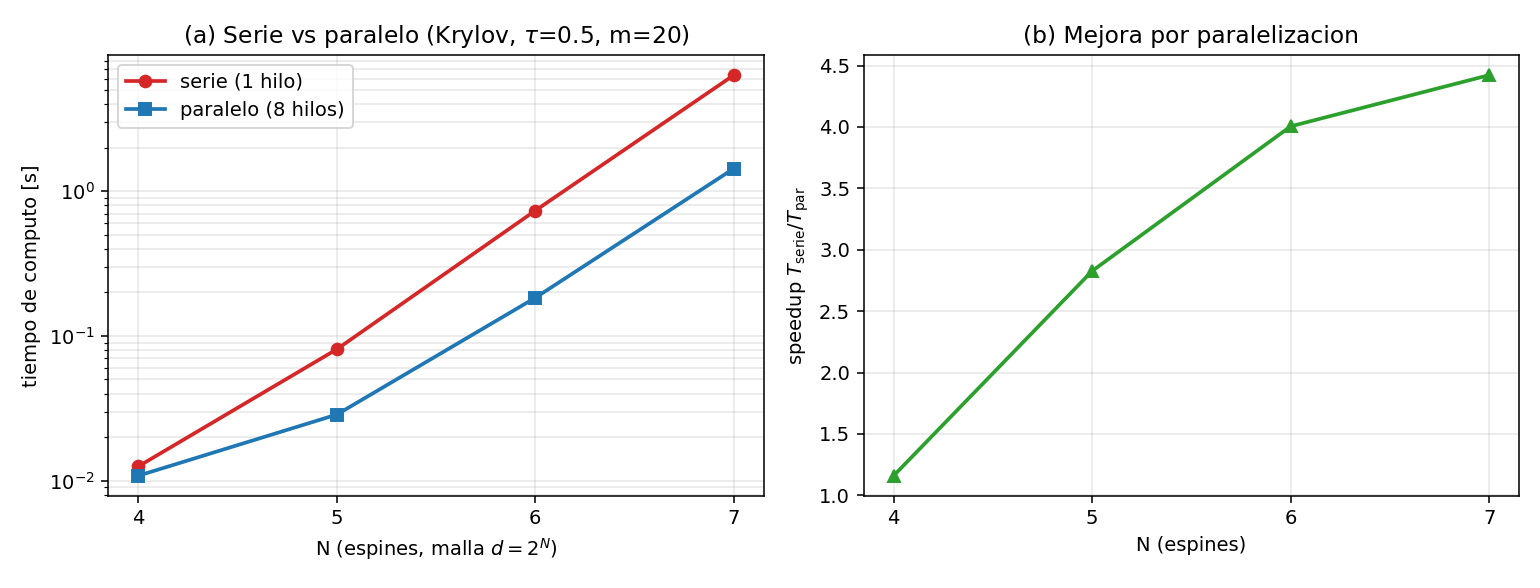
\includegraphics[width=0.92\textwidth]{../../T2/b_accion_exponencial/results/fig_t2b_serial_parallel.png}
\caption{Tiempo de cómputo \textbf{serie vs paralelo} del método de Krylov frente
al tamaño del sistema $N$ (malla $d=2^N$), a $\tau=0{,}5$ y $m=20$ fijos.
(a)~curvas de $1$~hilo (rojo) y $8$~hilos (azul) en escala log; (b)~speedup
$T_{\mathrm{serie}}/T_{\mathrm{par}}$ resultante. El patrón es el mismo que el de
RK4 porque el hotspot paralelo —el \texttt{matmul} de la acción de $\mathcal L$—
es común a ambos métodos.}
\label{fig:t2b_serial_parallel}
\end{figure}

\subsection{Comparación de método (a vs b): el resultado central}
La ventaja de Krylov no está en el escalado paralelo (idéntico al de RK4) sino en
el \textbf{trabajo necesario para una precisión dada}. La
figura~\ref{fig:t2b_method} mide el error del observable $D_{HS}$ final frente a
una referencia de alta precisión, en función del número de aplicaciones de
$\mathcal{L}$ (la operación cara, independiente de la máquina):

\begin{figure}[h]
\centering
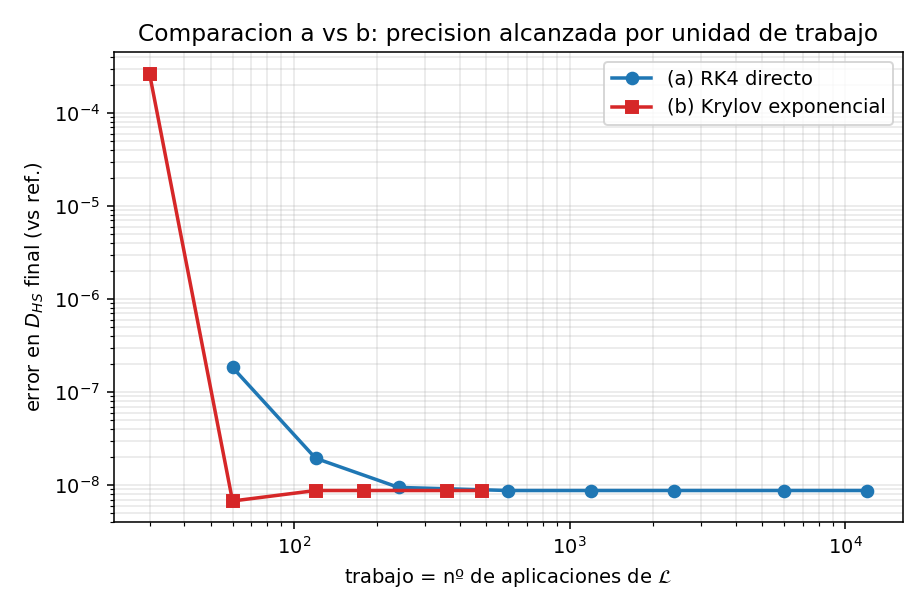
\includegraphics[width=0.7\textwidth]{../../T2/b_accion_exponencial/results/fig_t2b_method_compare.png}
\caption{Error del observable $D_{HS}$ final frente a la referencia exacta
(evolución espectral), en función del trabajo. \textbf{A igual trabajo
($\approx 60$ aplicaciones de $\mathcal{L}$), Krylov es $\sim$25$\times$ más
preciso} ($7\times10^{-9}$ frente a $2\times10^{-7}$ de RK4). El punto Krylov de
$m=10$ (no convergido, $2\times10^{-4}$) cae cinco órdenes de magnitud al pasar a
$m=20$: convergencia \emph{super-algebraica} en $m$, frente a la algebraica
($\propto\Delta t^4$) de RK4. El suelo $\sim 9\times10^{-9}$ es la precisión de
la propia referencia.}
\label{fig:t2b_method}
\end{figure}

La interpretación física/numérica: RK4 converge \emph{algebraicamente} (el error
baja como $\Delta t^4$), mientras que Krylov converge \emph{super-algebraicamente}
(casi exponencial en $m$) porque captura la acción exacta del exponencial dentro
del subespacio. En este sistema disipativo \emph{no rígido}, ambos métodos son de
trabajo comparable para precisiones moderadas, pero Krylov presenta tres ventajas
estructurales: (i)~a igual trabajo es $\sim$25$\times$ más preciso; (ii)~usa pasos
de tiempo $5\times$ mayores ($\tau=1{,}0$ frente a $\Delta t=0{,}2$) manteniéndose
estable y exacto; (iii)~es \textbf{incondicionalmente estable}, mientras que RK4
tiene un límite de estabilidad $\Delta t<2{,}8/|\lambda_{\max}|$. Esta ventaja se
vuelve \emph{decisiva} para generadores \emph{rígidos} (escalas de energía grandes
o disipación fuerte) y para alcanzar el estado estacionario, donde el límite de
estabilidad obliga a RK4 a dar muchísimos pasos diminutos. RK4 sigue siendo
preferible cuando se necesita la trayectoria \emph{densamente} muestreada en el
tiempo o cuando el Liouvilliano depende del tiempo.

\subsection{Resultados y conclusión del método (b)}
La figura~\ref{fig:t2b_relax} muestra la curva de relajación obtenida con pasos
\emph{grandes} ($\tau=0{,}25$), inalcanzables para RK4 a esa precisión. Resumen de
la comparación a--b:
\begin{itemize}[leftmargin=1.6em,itemsep=1pt]
\item Misma física (resultados idénticos), misma paralelización (OpenMP sobre
\texttt{matmul}, escalado sublineal equivalente).
\item Krylov~(b): mucho menos trabajo para alta precisión y pasos de tiempo
grandes; ideal para llegar al estacionario o muestrear pocos tiempos.
\item RK4~(a): más simple, robusto, y mejor para trayectorias densas o
generadores dependientes del tiempo.
\end{itemize}

\begin{figure}[h]
\centering
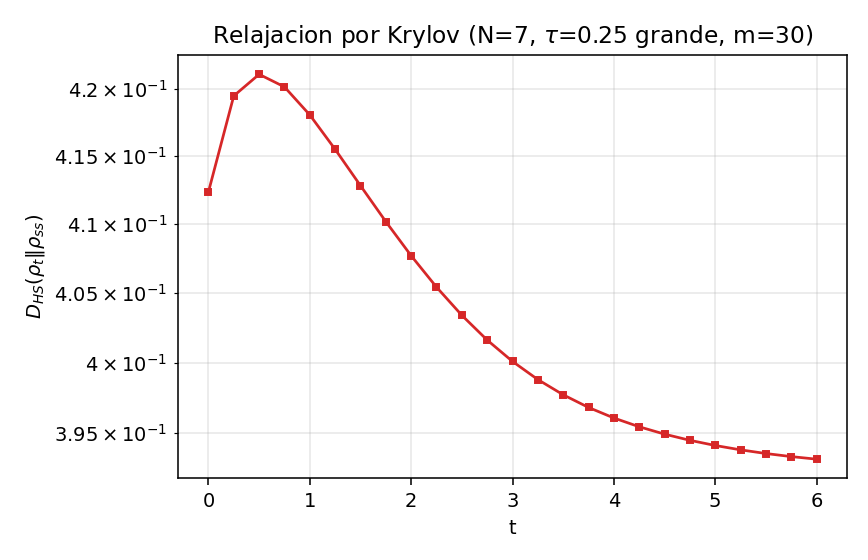
\includegraphics[width=0.6\textwidth]{../../T2/b_accion_exponencial/results/fig_t2b_relax.png}
\caption{Relajación $D_{HS}(t)$ por Krylov con pasos grandes $\tau=0{,}25$
($N=7$), medida al \textbf{estado estacionario verdadero} $\rss$ (núcleo de
$\Lop$): por eso baja a $0$.}
\label{fig:t2b_relax}
\end{figure}

\subsection{El efecto Mpemba: cruce de curvas}
El método de Krylov reproduce el efecto Mpemba con idéntica física que RK4 (ambos
resuelven la misma ecuación maestra). La Figura~\ref{fig:t2b_mpemba} evoluciona por
Krylov dos preparaciones del mismo Ising disipativo: $\ket{+}^{\otimes N}$ (parte
lejos) y $\ket{0}^{\otimes N}$ (parte cerca), midiendo la distancia al estado
estacionario verdadero $\rss$. La que parte lejos \textbf{adelanta} a la otra en
$t^*\approx0{,}69$ —el mismo $t^*$ que da RK4 (\S\ref{sec:t2a}), confirmando que el
cruce es físico y no del integrador.

\begin{figure}[h]
\centering
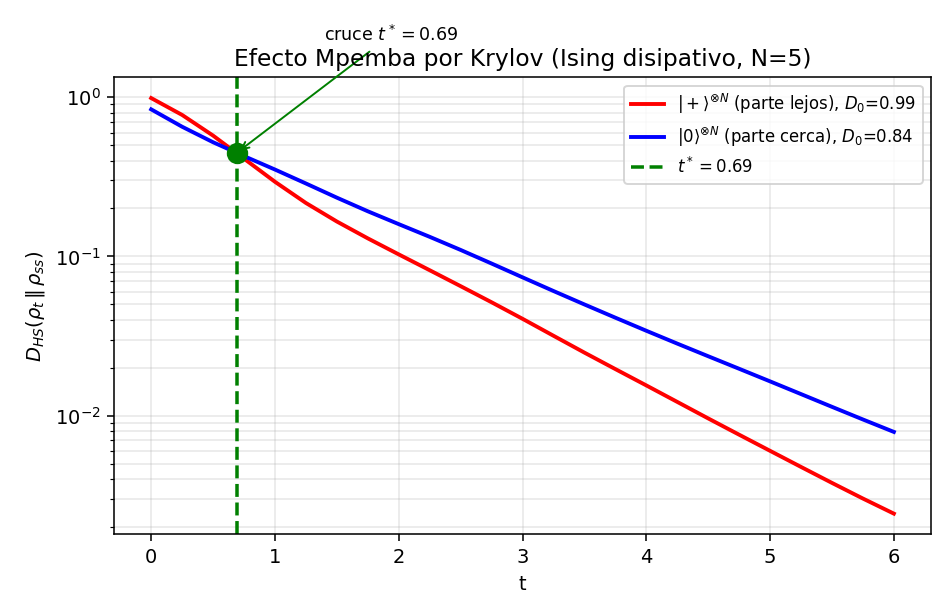
\includegraphics[width=0.72\textwidth]{../../T2/b_accion_exponencial/results/fig_t2b_mpemba.png}
\caption{Efecto Mpemba por Krylov (Ising disipativo, $N=5$). $D_{HS}(t)$ a $\rss$
para $\ket{+}^{\otimes N}$ (roja, lejos) y $\ket{0}^{\otimes N}$ (azul, cerca): la
roja cruza a la azul en $t^*\approx0{,}69$, idéntico al de RK4.}
\label{fig:t2b_mpemba}
\end{figure}

% =====================================================================
%  Entregable T3(a): Muchos cuerpos por trayectorias cuanticas (MPI)
%  Fragmento \input-able en context/doc/mpemba_cuantico.tex
% =====================================================================
\section{Muchos cuerpos: trayectorias cuánticas con MPI}
\label{sec:t3}

\subsection{Explicación del framework}
En el régimen de \emph{muchos cuerpos} la representación densa del operador
densidad $\rho$ se vuelve inviable: para $N$ qubits, $\rho$ tiene $d^2=4^N$
elementos y el Liouvilliano $4^N\times4^N$. El método de \textbf{trayectorias
cuánticas} (\emph{Monte Carlo wavefunction}, MCWF) sortea este muro: en lugar de
propagar $\rho$, propaga $M$ \emph{vectores de estado puros}
$\ket{\psi}\in\mathbb{C}^{d}$ y recupera el operador densidad como promedio
estocástico
\[
\rho(t)=\mathbb{E}\big[\dyad{\psi(t)}{\psi(t)}\big]\;\approx\;\frac1M\sum_{j=1}^{M}\dyad{\psi_j(t)}{\psi_j(t)}.
\]
Esto reduce la memoria de $d^2$ a $d$ y, sobre todo, convierte el problema en uno
\textbf{embarrassingly parallel}: cada trayectoria es independiente.

\subsection{Del modelo teórico a la discretización (paso a paso)}
\label{ssec:t3_discr}

\paragraph{Paso 0 — Modelo teórico.} El mismo generador GKSL
$\dot\rho=\Lop[\rho]$ de la cadena de Ising disipativa (\S\ref{ssec:t2a_discr}).

\paragraph{Paso 1 — \emph{Unraveling} estocástico.} En vez de propagar $\rho$, se
reescribe la ecuación maestra como un promedio sobre \emph{trayectorias} de
estados puros (\emph{Monte Carlo wavefunction}, Dalibard--Mølmer--Castin):
$\rho(t)=\mathbb{E}\big[\dyad{\psi(t)}{\psi(t)}\big]$. La parte coherente más la
parte ``de no salto'' del disipador se agrupan en un \textbf{Hamiltoniano efectivo
no hermítico}
\[
H_{\mathrm{eff}}=H-\tfrac{i}{2}\sum_\mu L_\mu^\dagger L_\mu,
\]
cuya evolución $\dot{\ket\psi}=-iH_{\mathrm{eff}}\ket\psi$ \emph{no} conserva la
norma; el defecto de norma es exactamente la probabilidad de salto.

\paragraph{Paso 2 — Discretización temporal de cada trayectoria.} Con paso
$\Delta t$, cada trayectoria alterna:
\begin{enumerate}[leftmargin=1.6em,itemsep=1pt]
\item \textbf{Evolución determinista} $\dot{\ket\psi}=-iH_{\mathrm{eff}}\ket\psi$ por
\textbf{RK4} (4.º orden; elimina el sesgo $\mathcal{O}(\Delta t)$ de un Euler
ingenuo). Resulta $\psi'$ con $\|\psi'\|^2=1-\delta p$.
\item \textbf{Salto estocástico.} Probabilidad $\delta p=1-\|\psi'\|^2$; se sortea
$\varepsilon\sim U(0,1)$: si $\varepsilon<\delta p$ hay \emph{salto} (se elige el
canal $\mu$ con probabilidad $\propto\|L_\mu\psi\|^2$ y
$\ket\psi\leftarrow L_\mu\ket\psi/\|L_\mu\psi\|$); si no,
$\ket\psi\leftarrow\psi'/\|\psi'\|$.
\end{enumerate}

\paragraph{Paso 3 — Promedio de conjunto.} El observable se recupera promediando
las $M$ trayectorias,
$\rho(t)\approx\frac1M\sum_{j=1}^{M}\dyad{\psi_j(t)}{\psi_j(t)}$. Coste por paso:
unos pocos productos matriz--vector $\mathcal{O}(d^2)$ (no $\mathcal{O}(d^3)$);
precisión del promedio $\propto M^{-1/2}$. \emph{Las $M$ trayectorias son
independientes} $\Rightarrow$ el promedio es la única operación colectiva
(Paso~3 $=$ una \texttt{MPI\_Reduce}).

\subsection{Implementación serial y líneas de código}
En \texttt{T3/integration/src/trajectories\_mpi.cpp} (reutiliza
\texttt{T2/common/lindblad.hpp} para el modelo y \texttt{matvec}). El estado
inicial es el puro $\ket{0}$ y la referencia el Gibbs del baño. Cada trayectoria
usa un generador \texttt{mt19937\_64} sembrado con su índice \emph{global}, lo que
hace el resultado \textbf{reproducible e independiente del número de rangos}. El
Paso~2 (no-salto vs salto) es literalmente:

\begin{lstlisting}[language=C++,caption={Decisión determinista/salto por trayectoria (\texttt{trajectories\_mpi.cpp}). \texttt{psip} es el estado tras el paso RK4 de $H_{\mathrm{eff}}$; \texttt{norm2}$=\|\psi'\|^2$.},label={lst:t3_jump}]
double dp = 1.0 - norm2;                              // probabilidad de salto
if (U(rng) < dp) {                                    // --- SALTO ---
    /* elegir canal mu con prob ~ ||L_mu psi||^2 ... */
    std::vector<cd> Lp = matvec(Ls[mu], psi, d);
    for (int a = 0; a < d; ++a) psi[a] = Lp[a] / nn;  // psi <- L_mu psi / ||.||
} else {                                              // --- NO salto: renormalizar ---
    double inv = 1.0 / std::sqrt(norm2);
    for (int a = 0; a < d; ++a) psi[a] = psip[a] * inv;
}
\end{lstlisting}

\subsection{Las llamadas de paralelización (MPI)}
El paralelismo es de \emph{tareas}: cada rango calcula su lote de trayectorias sin
comunicación, y una sola reducción promedia. Las tres líneas MPI que estructuran
todo el cálculo son el arranque, el reparto y la reducción final:

\begin{lstlisting}[language=C++,caption={Esqueleto MPI de \texttt{trajectories\_mpi.cpp}: arranque e identificación del rango, reparto balanceado de las $M$ trayectorias entre rangos (sin comunicación), y la \emph{única} operación colectiva \texttt{MPI\_Reduce} que suma los acumuladores en el rango 0 (Paso~3, el promedio).},label={lst:t3_mpi}]
MPI_Init(&argc, &argv);                       // arranque del entorno MPI
MPI_Comm_rank(MPI_COMM_WORLD, &rank);         // id de este rango
MPI_Comm_size(MPI_COMM_WORLD, &size);         // numero total de rangos
// ... reparto balanceado de las M trayectorias (embarrassingly parallel):
int per = M / size, rem = M % size;
int my_M = per + (rank < rem ? 1 : 0);        // cuantas calcula este rango
int my_start = rank * per + std::min(rank, rem);
// ... cada rango integra sus my_M trayectorias en un acumulador local 'acc' ...
// UNICA comunicacion: sumar los acumuladores locales -> rho(t) en el rango 0
MPI_Reduce(reinterpret_cast<double*>(acc.data()),
           rank == 0 ? reinterpret_cast<double*>(glob.data()) : nullptr,
           (int)(2 * acc.size()), MPI_DOUBLE, MPI_SUM, 0, MPI_COMM_WORLD);
\end{lstlisting}

\subsection{Justificación de la paralelización: MPI}
El patrón de cómputo es radicalmente distinto al de la evolución temporal (T2):
no hay una larga cadena de pasos dependientes sobre un único objeto grande, sino
$M$ cálculos \emph{completamente independientes} sobre objetos pequeños
($\ket\psi\in\mathbb{C}^d$), seguidos de una \emph{única reducción} (el promedio).
Este es el caso de libro del paradigma \textbf{MPI} de paralelismo de tareas:
cada rango calcula su lote de trayectorias sin comunicación alguna y al final una
sola \texttt{MPI\_Reduce} promedia los acumuladores. No hay comunicación de halo
ni dependencias, por lo que el escalado es \emph{casi ideal} y \emph{multinodo}
(a diferencia de OpenMP, limitado a un nodo y al ancho de banda compartido).
CUDA sería un acelerador complementario \emph{dentro} de cada rango (evolucionar
cientos de trayectorias en lote en una GPU), pero el reparto grueso natural es
MPI. La corrección se verifica de dos formas: (i)~el resultado es idéntico con
1, 4 u 8 rangos (misma semilla por índice global $\Rightarrow$ reducción
correcta); (ii)~el promedio reproduce la ecuación maestra exacta (validación
abajo).

\subsection{Comparación serial vs paralelo}
\begin{figure}[h]
\centering
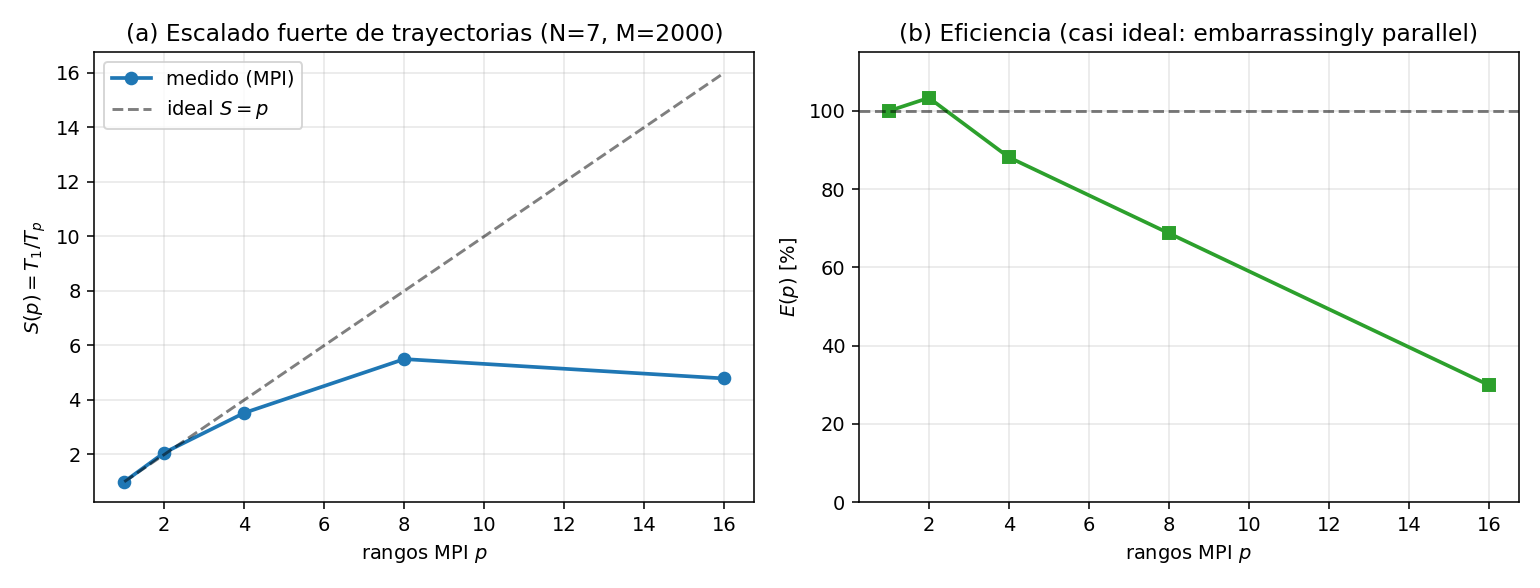
\includegraphics[width=0.92\textwidth]{../../T3/integration/results/fig_t3_speedup.png}
\caption{Escalado fuerte de las trayectorias cuánticas sobre rangos MPI
($N=7$, $M=2000$ fijo). El speedup es \textbf{casi ideal}
($S_{\max}\approx5{,}5$ con $8$ rangos, eficiencia $69\,\%$),
en marcado contraste con el escalado sublineal del OpenMP de la evolución
temporal (T2, $S\approx2{,}9$--$3{,}3$). La razón: ausencia total de
comunicación y dependencias entre trayectorias.}
\label{fig:t3_speedup}
\end{figure}

\textbf{Contraste de paradigmas (el resultado clave del reparto T2 vs T3).} La
evolución temporal (T2) paraleliza \emph{dentro} de un paso con OpenMP y satura
pronto (memoria compartida, ancho de banda, fork/join): $S\!\lesssim\!3{,}3$. Las
trayectorias (T3) paralelizan \emph{entre} tareas independientes con MPI y escalan
casi linealmente: $S\approx5{,}5$. Es la ilustración perfecta de que el
paradigma óptimo lo dicta el \emph{patrón de cómputo}, no una preferencia a
priori.

La Figura~\ref{fig:t3_serial_parallel} hace explícita la mejora variando el
parámetro propio del método —el \textbf{número de trayectorias $M$}, que fija el
trabajo Monte Carlo— y enfrentando el \textbf{tiempo en serie (1~rango) y en
paralelo (8~rangos)}. Ambas crecen linealmente con $M$ (coste $\propto M$), pero
con pendientes muy distintas: las rectas \emph{divergen}, y el cociente entre
ellas se mantiene casi constante y cercano al número de núcleos, precisamente
porque no hay comunicación entre trayectorias.

\begin{figure}[h]
\centering
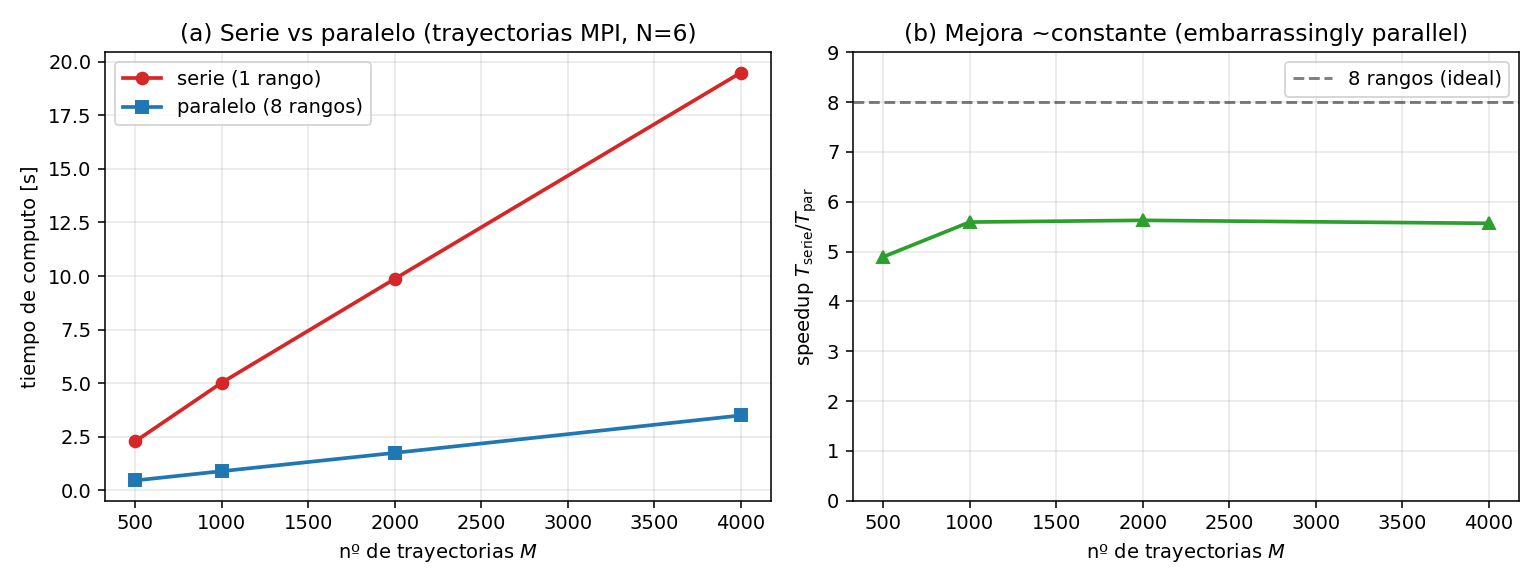
\includegraphics[width=0.92\textwidth]{../../T3/integration/results/fig_t3_serial_parallel.png}
\caption{Tiempo de cómputo \textbf{serie vs paralelo} de las trayectorias frente
al número de trayectorias $M$ ($N=6$, $d=64$). (a)~serie ($1$~rango, rojo) y
paralelo ($8$~rangos, azul) crecen como $\propto M$ con pendientes distintas: el
hueco —la mejora— se ensancha con $M$. (b)~el speedup
$T_{\mathrm{serie}}/T_{\mathrm{par}}$ es \emph{casi constante} en $M$ (línea de
referencia ideal $=8$), firma del paralelismo \emph{embarrassingly parallel}.}
\label{fig:t3_serial_parallel}
\end{figure}

\subsection{Resultados y validación}
\paragraph{Convergencia estadística.}
La figura~\ref{fig:t3_error} muestra que el error del observable $D_{HS}$ final frente a
la ecuación maestra exacta (evolución espectral desde $\ket{0}$,
$D_{HS}^{\text{exacto}}=0{,}40490$) decae como $M^{-1/2}$ (pendiente medida
$\approx-0{,}6$, consistente con $M^{-1/2}$), confirmando la convergencia de Monte Carlo. El uso de RK4 en
la parte determinista elimina el sesgo sistemático: a $\Delta t=0{,}02$ y
$M=8000$ el resultado coincide con el exacto con una diferencia de $\sim0{,}002$.

\begin{figure}[h]
\centering
\begin{minipage}{0.49\textwidth}\centering
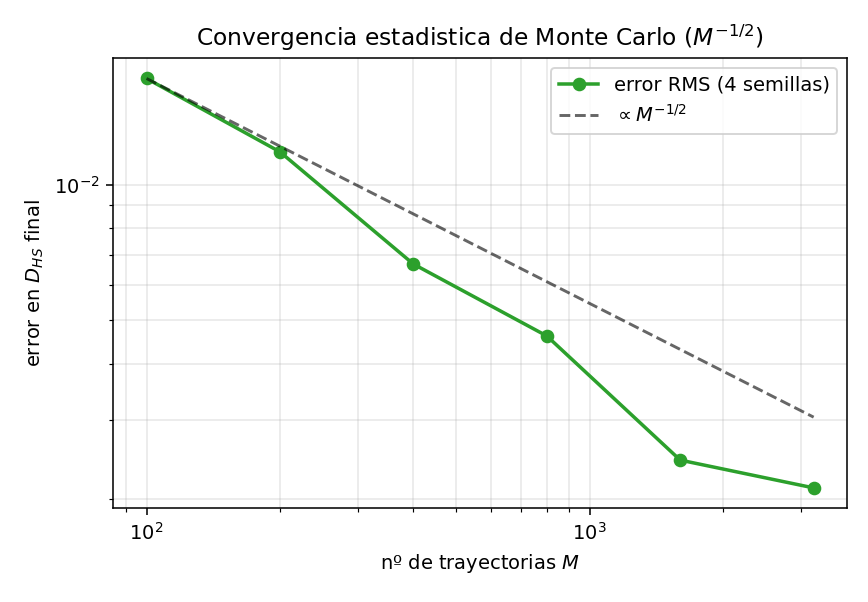
\includegraphics[width=\textwidth]{../../T3/integration/results/fig_t3_error_M.png}
\end{minipage}\hfill
\begin{minipage}{0.49\textwidth}\centering
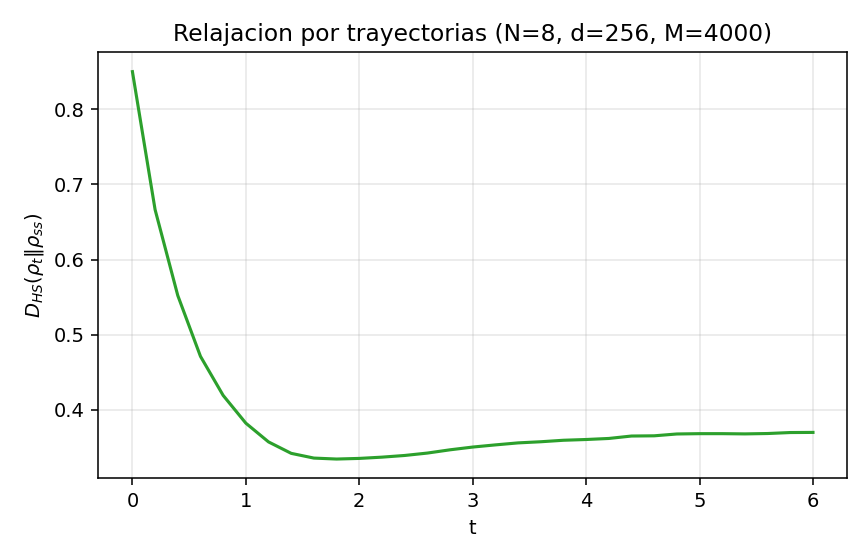
\includegraphics[width=\textwidth]{../../T3/integration/results/fig_t3_relax.png}
\end{minipage}
\caption{Izquierda: convergencia estadística $M^{-1/2}$ del promedio de
trayectorias. Derecha: curva de relajación $D_{HS}(t)$ para $N=8$ ($d=256$,
$M=4000$), un sistema en el que el método de trayectorias usa vectores de $256$
componentes en lugar de operadores densidad de $256^2$.}
\label{fig:t3_error}
\end{figure}

\paragraph{Conclusión del método de trayectorias.}
Las trayectorias cuánticas son el método de elección para muchos cuerpos: memoria
$\mathcal{O}(d)$ por trayectoria, coste $\mathcal{O}(d^2)$ por paso y, sobre todo,
\textbf{escalado MPI casi ideal} que aprovecha clústeres multinodo. El precio es
la convergencia $M^{-1/2}$ (para una cifra más de precisión hacen falta $100\times$
trayectorias), mitigable precisamente por la abundancia de paralelismo. Para
cadenas largas y observables de entrelazamiento, el relevo natural son las redes
tensoriales (entregable de Juan, \S\ref{sec:t3b}).

% =====================================================================
%  Entregable 8: Influencia y relevancia en el efecto macro clasico
%  Fragmento \input-able en context/doc/mpemba_cuantico.tex
% =====================================================================
\section{Influencia y relevancia en el efecto macroscópico clásico}
\label{sec:macro}

\subsection{La raíz macroscópica y su problema histórico}
El efecto Mpemba nació como una observación \emph{macroscópica y clásica}: agua
inicialmente más caliente que se congela antes que agua más fría
(Mpemba--Osborne 1969). Durante medio siglo fue un fenómeno disputado, porque a
escala macroscópica intervienen muchos mecanismos difíciles de controlar
(convección, evaporación, sobreenfriamiento, gases disueltos) y porque
\emph{carecía de un criterio teórico limpio}: ¿qué significa exactamente que un
sistema esté ``más lejos del equilibrio''? Distintas métricas de distancia daban
respuestas distintas (la crítica de Burridge--Linden 2016).

\subsection{El mecanismo unificador: geometría espectral de la relajación}
El marco cuántico desarrollado en este trabajo aporta, precisamente, lo que le
faltaba al fenómeno macroscópico: un \textbf{mecanismo espectral riguroso} que es
\emph{el mismo} en el régimen clásico y en el cuántico. En ambos casos la
relajación se descompone en modos,
\[
\text{clásico: } \vb{p}(t)=\pi+\sum_{k\ge2} a_k\, e^{\lambda_k t}\,\vb{v}_k,
\qquad
\text{cuántico: } \rho(t)=\rss+\sum_{k\ge2} a_k\, e^{\lambda_k t}\,\hat r_k,
\]
con $\vb{v}_k$ los autovectores de la matriz de tasas y $\hat r_k$ los
autooperadores del Liouvilliano. El efecto Mpemba ocurre, en \emph{los dos}
mundos, cuando la preparación caliente \emph{solapa poco con el modo lento}
($a_2\approx0$): es un fenómeno de \textbf{geometría no-normal} de los modos de
relajación, no una propiedad del agua. Lo que en el agua era una anomalía
empírica resulta ser un caso particular de una estructura matemática general.

\subsection{Lo que el enfoque cuántico devuelve al problema clásico}
Tres aportaciones del marco cuántico iluminan directamente el efecto macroscópico:
\begin{enumerate}[leftmargin=1.7em,itemsep=2pt]
\item \textbf{Criterio espectral del Mpemba fuerte} ($a_2=0$, Carollo \emph{et
al.}): da una condición \emph{exacta} y constructiva para la aceleración, válida
también para sistemas clásicos de muchos estados (vidrios, granulares).
\item \textbf{Diagnóstico independiente de la métrica} (termomayorización,
Vu--Hayakawa): resuelve la ambigüedad histórica de Burridge--Linden ---certifica
el efecto bajo \emph{todas} las distancias monótonas a la vez--- y es aplicable
tal cual a las distribuciones clásicas.
\item \textbf{Los puntos excepcionales y el recurso metrológico}: conceptos
nacidos en el régimen cuántico que sugieren nuevos protocolos (aceleración por
preparación, termometría fuera del equilibrio) trasladables a plataformas
clásicas controladas.
\end{enumerate}

\subsection{La firma universal: del macro clásico al cuántico}
La figura~\ref{fig:macro} muestra la \emph{misma} firma ---el cruce de las curvas de
relajación, donde una preparación que parte más lejos alcanza el equilibrio
antes--- en tres dominios físicos usando los datos del repositorio: un coloide
clásico en trampa óptica (Kumar 2022), un circuito cuántico de muchos cuerpos
(Turkeshi 2024) y la simulación cuántica propia de este trabajo. La continuidad
conceptual es total: el mismo criterio de solapamiento espectral explica el cruce
en los tres casos.

\begin{figure}[h]
\centering
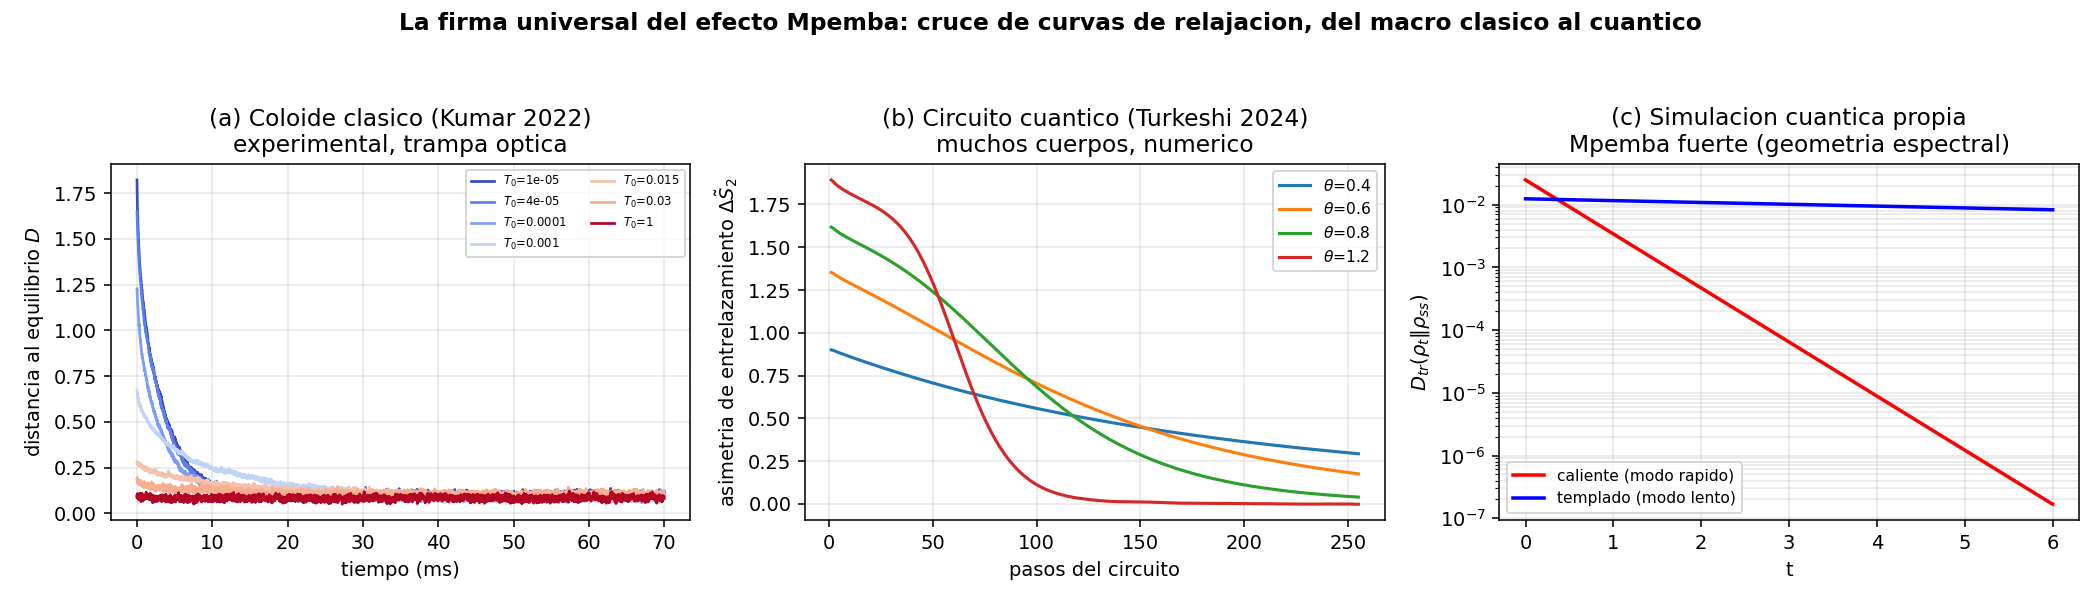
\includegraphics[width=\textwidth]{../../macro/results/fig_macro_universal.png}
\caption{La firma universal del efecto Mpemba ---el cruce de curvas de
relajación--- del macro clásico al cuántico. (a)~coloide clásico experimental
(Kumar 2022): la distancia al equilibrio de una preparación caliente cruza por
debajo de otra más fría. (b)~circuito cuántico de muchos cuerpos (Turkeshi 2024):
la asimetría de entrelazamiento de $\theta=1{,}2$ parte como la mayor pero se
restaura antes. (c)~simulación cuántica propia (Mpemba fuerte por geometría
espectral). El mecanismo ---solapamiento con los modos lentos--- es común.}
\label{fig:macro}
\end{figure}

\subsection{Relevancia}
La relevancia es doble. \emph{Hacia atrás}: el aparato cuántico
(modos del generador, solapamientos, diagnósticos universales) proporciona al
efecto macroscópico clásico el fundamento teórico riguroso que históricamente le
faltó, convirtiendo una curiosidad sobre el agua en un teorema sobre la
relajación fuera del equilibrio. \emph{Hacia adelante}: muestra que el mismo
fenómeno, y las mismas herramientas computacionales (descomposición espectral,
evolución del operador densidad, trayectorias), abarcan sin costura desde el vaso
de agua hasta el procesador cuántico, lo que justifica tratar el efecto Mpemba
como un \emph{principio general de diseño} de protocolos de relajación acelerada.


\end{document}
